\documentclass[12]{article}
\usepackage{graphicx}
\begin{document}
\begin{titlepage}
\begin{center}
\begin{Large}
\textbf{Assignment-6} \\
\medskip
\bigskip
\textbf{ELP - 718 Telecom Software Laboratory}\\
\end{Large}
\bigskip

\begin{large}
\textbf{Ankit Dixit}\\
\medskip
\textbf{2017JTM2769}\\
\medskip
\textbf{semester-1}
\end{large}
\bigskip
\bigskip\\
\begin{large}
A report presented for the assignment \\
\medskip
Developing logical skills to solve the given problem with the help of basics of Python\\
\end{large}

\vspace{3.5cm}

\includegraphics[scale=0.5]{logo} \\
\medskip
\bigskip
\bigskip
\begin{large}
\textbf{
Bharti School Of \\
\medskip
Telecommunication Technology and Management \\
\medskip
IIT DELHI\\
\smallskip
India\\
}
\bigskip
\textbf{\today}
\end{large}
\end{center}
\end{titlepage}





\newpage
\tableofcontents



\newpage
\section{Problem Statement-1}

\subsection{Problem statement} 
Write a code in python for displaying the message frame along with the parity checking i.e.odd parity check and then after the bit stuffing based on the rule given in the assumptions.

\subsection{Assumptions}
\begin{itemize}
\item \textbf{Parity Check} \\
The simplest way of error detection is to append a single bit , called a parity check, to a string of data bits. This parity check bit has the value 1 if number of 1’s in the bit string is even and has the value 0 otherwise, i.e., Odd Parity Check.
\item \textbf{Bit Oriented Framing} \\
Data Link Layer needs to pack bits into frames, so that each frame is distinguishable from another. Frames can be fixed or variable size. In variable size framing, we define end of frame using bit oriented approach. It uses a special string of bits, called a flag for both idle fill and to indicate the beginning and the ending of frames.
The string 0101 is used as the bit string or flag to indicate the end of the frame. The bit stuffing rule is to insert a 0 after each appearance of 010 in the original data. In addition, if the frame ends in 01, a 0 would be stuffed after the 1st 0 in the actual terminating string 0101.

\end{itemize}
\subsection{Program structure}
\begin{itemize}
\item first part of the programme we take input from the user and store them
\item then store them into a list and apply the logic to calculate the bits that is to be stuffed and parity bit.
\item after the the calculation merge the list element that is append the same list with extra element.
\item then finaaly show the output.
\end{itemize}
\subsection{Algorithm and Implementation}
\begin{itemize}
\item take no of bits in mesage from the user.
\item then store them into a list.
\item calculate the parity bit.
\item stuff this into the same list.
\item now check for the condition that is given and stuff the bit based on it.
\item now finally print the list.
\end{itemize}
\subsection{Input and Output format}
\textbf{Input Format} \\
Enter binary bit data which has to be transmitted. \\


\textbf{Output Format} \\
Print binary bit data with parity bit.\\
Print the modified string received at the other end. \\


\subsection{Test cases}
\textbf{Sample Input}\\
01010 \\

\textbf{Sample Output} \\
010101 \\ 
0100100100101 \\

\subsection{Difficulties /Issues faced}
\begin{itemize}
\item over indexing.
\item logic development.
\item format error.
\item syntsx error.
\end{itemize}
\subsection{Screenshots}
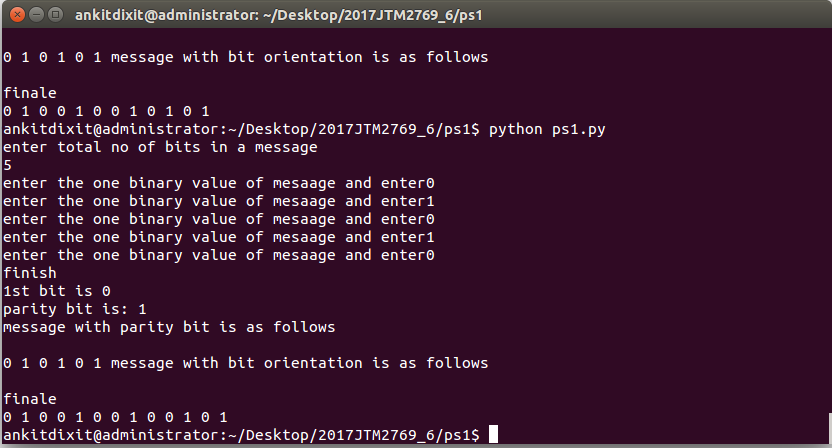
\includegraphics[scale=0.5]{ps1.png}

\newpage
\section{Problem Statement-2}

\subsection{Problem statement} 
3X3 Numeric Tic-Tac-Toe (Use numbers 1 to 9 instead of X’s and O’s)
One player plays with the odd numbers (1, 3, 5, 7, 9) and other player plays with the even numbers (2,4,6,8). All numbers can be used only once. The player who puts down 15 points in a line wins (sum of 3 numbers). Always Player with odd numbers start the game. Once a line contains two numbers whose sum is 15 or greater, there is no way to complete that line, although filling in the remaining cell might be necessary to complete a different line. \\
Note – Line can be horizontal, vertical or diagonal


\subsection{Assumptions}
\textbf{Constraints:}
\begin{itemize}
\item 1 $<= Position<=9$
\item $1<=Number<=9$
\item $1<=Sum<=15$
\end{itemize}


\subsection{Program structure}
\begin{itemize}
\item We define the users 
\item then after defineing the users take their preference and allot them the values
\item check for the constraints at the time of input and then perform it.
\end{itemize}
\subsection{Algorithm and Implementation}

\subsection{Input and Output format}
\begin{itemize}
\item \textbf{Input format}\\ 
input is in the form of numerics.
\item \textbf{Output format} \\
output is in the form of text that whether you wins or not.
\end{itemize}
\subsection{Test cases}
\textbf{Sample Output:} \\
Welcome to the Game! \\
Player 1’s chance \\
Enter the position and number to be entered: 5,3 \\








 3


 




\\
Player 2’s chance \\
Enter the position and number to be entered: 7,4 \\









 3


 4




\\
... Continue till game ends \\
Note – Must use at least one User Defined Function. \\

\subsection{Difficulties /Issues faced}
\begin{itemize}
\item over indexing.
\item logic development.
\item format error.
\item syntsx error.
\end{itemize}
\subsection{Screenshots}
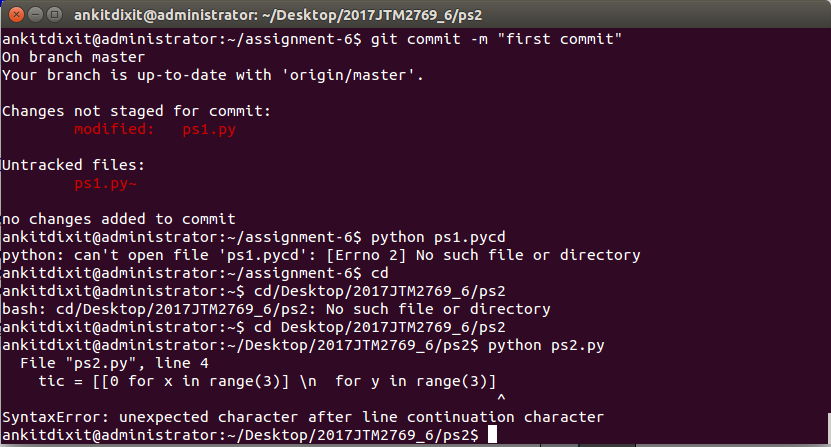
\includegraphics[scale=0.5]{ps2.png}

\newpage
\section*{Appendix}

\newpage
\section{References}
\begin{itemize}
\item let us C.
\item https://help.gnome.org/users/gedit/stable/
\item http://fresh2refresh.com/c-programming/c-data-types/
\item https://www.tutorialspoint.com/python/python_lists.htm
\item https://help.github.com/articles/fork-a-repo/
\item https://stackoverflow.com/questions/11119632/bitwise-xor-of-hex-numbers-in-python
\item http://www.physics.nyu.edu/pine/pymanual/html/chap3/chap3_arrays.html
\end{itemize}

\end{document}